\section{Doc Supplémentaire}

%-----------------------
\subsection{Références supplémentaires}

\begin{frame}
  \frametitle{Pour aller plus loin}
  Chercher de l'information:
    \begin{itemize}
        \item \url{http://en.wikibooks.org/wiki/LaTeX}
        \item \url{http://www.grappa.univ-lille3.fr/FAQ-LaTeX}
            \item \url{http://www.andy-roberts.net/writing/latex}
            \item \url{http://ctan.org/pkg/packagename} ou \lstinline[language=sh,morekeywords={texdoc}]{$ texdoc packagename}
        \item Google est ton ami !
            \item \url{https://www.overleaf.com/learn}
            \item La version de StackExchange spécialisée pour le \TeX:
  \url{https://tex.stackexchange.com}.
        \item Livres:
        \begin{itemize}
            \item \LaTeX HowTo par Sébastien Combéfis (EN/FR)
            \item Framabook \LaTeX
        \end{itemize}
    \end{itemize}
\end{frame}

%-----------------------
\subsection{L'Environnement Description}

\begin{frame}[fragile]
  \frametitle{Description}
  \begin{itemize}
    \item L'environnement \lstinline|description| permet de faire des définitions.
    \begin{lstlisting}[style=nonumbers]
\begin{description}
  \item[ODT] Open Document Text.
  \item[ODS] Open Document Spreadsheet.
  \item[ODP] Open Document Presentation.
\end{description}
    \end{lstlisting}
    \begin{description}
      \item[ODT] Open Document Text.
      \item[ODS] Open Document Spreadsheet.
      \item[ODP] Open Document Presentation.
    \end{description}
  \end{itemize}
\end{frame}

%-----------------------
\subsection{La Chimie}

\begin{frame}[fragile]
  \centering
  \frametitle{La chimie}
  \begin{lstlisting}
\usepackage{chemfig}
...
\chemfig{*6(-=(-CH_2OH)-(-COOH)=-=)}
  \end{lstlisting}
  \begin{center}
    \chemfig{*6(-=(-CH_2OH)-(-COOH)=-=)}
  \end{center}
  \begin{lstlisting}
\usepackage[version=3]{mhchem}
...
  \[\ce{3H2O + 1/2H2O -> AgCl2- + H2_{(aq)}}\]
  \end{lstlisting}
  \[\ce{3H2O + 1/2H2O -> AgCl2- + H2_{(aq)}}\]
\end{frame}

%-----------------------
\subsection{Les Circuits}

\begin{frame}[fragile]
  \frametitle{Les circuits}
  \begin{lstlisting}
\usepackage{circuitikz}
...
\shorthandoff{:!} % Pour certaines versions de circuitikz
\begin{circuitikz}
  \draw (0,0) to [sI, v=$V_2$] (0,-3);
  \draw (6,-3) to[short, i = $I_2$] (0,-3);
  \draw (0,0) to [R = R, v = $V_R$] (3,0);
  \draw (3,0) to [L = L, v = $V_L$] (6,0);
  \draw (6,0) to [C = C, v = $V_C$] (6,-3);
\end{circuitikz}
\shorthandon{:!} % Pour certaines versions de circuitikz\end{lstlisting}
  \begin{center}
        \shorthandoff{:!}
    \begin{circuitikz}
      \draw (0,0) to [sI, v=$V_2$] (0,-3);
      \draw (6,-3) to[short, i = $I_2$] (0,-3);
      \draw (0,0) to [R = R, v = $V_R$] (3,0);
      \draw (3,0) to [L = L, v = $V_L$] (6,0);
      \draw (6,0) to [C = C, v = $V_C$] (6,-3);
    \end{circuitikz}
        \shorthandon{:!}
  \end{center}
\end{frame}

%-----------------------
\subsection{Inclure du Code}

\begin{frame}[fragile]
  \frametitle{Inclure du code}
  \begin{lstlisting}[mathescape=true]
\begin{lstlisting}
if a == b:
  return 0
else:
  return 1
\$\color{blue}{\texttt{end}}${lstlisting}\end{lstlisting}
donne
  \begin{lstlisting}[language=Python]
if a == b:
  return 0
else:
  return 1\end{lstlisting}

  Il y a aussi
  \begin{lstlisting}
\lstinputlisting[caption={...},label=...]{main.py}\end{lstlisting}
  et
  \begin{lstlisting}
\lstinline|if a == b|\end{lstlisting}
  qui donne \lstinline|if a == b|.
\end{frame}

%-----------------------

\begin{frame}[fragile]
  \frametitle{Minted}

  \begin{itemize}
    \item Sur Overleaf : tout est déjà prêt pour minted
    \item Sur votre pc (en local) :
    \begin{enumerate}
      \item Ajouter --shell-escape aux paramètres de compilation
      \item Besoin du package python pygmentize
    \end{enumerate}
  \end{itemize}

  \begin{lstlisting}[mathescape=true]
    \begin{minted}{python}
      def dummy_function(count):
          i = 0
          while i < count:
            print("Affiche du code de façon simple")
    \end{minted}\end{lstlisting}

  Ceci donne :

  \begin{minted}{python}
    def dummy_function(count):
        i = 0
        while i < count:
          print("Affiche du code de façon simple")
  \end{minted}
\end{frame}

%-----------------------
\subsection{Dessiner en LaTeX avec Tikz}

\begin{frame}[fragile]
  \frametitle{Dessiner en LaTeX avec Tikz}
  \begin{figure}[!ht] \centering
    \includegraphics[width=0.8\textwidth]{img/turbine}
  \end{figure}
\end{frame}

%-----------------------
\subsection{Taille de Police}

\begin{frame}[fragile]{Jouer avec la police}
  \framesubtitle{Changer la taille de police}
  \begin{itemize}
      \item \lstinline|{\small text}| pour changer la taille du texte à l'intérieur
      \item \lstinline|\small| pour changer tout le texte jusqu'au prochain appel de \lstinline|\normalsize|
  \end{itemize}
  \begin{tabular}{ll}
  \lstinline|{\tiny polygenelubricants}| & {\tiny polygenelubricants} \\
  \lstinline|{\small polygenelubricants}| & {\small polygenelubricants} \\
  \lstinline|{\normalsize polygenelubricants}| & {\normalsize polygenelubricants} \\
  \lstinline|{\large polygenelubricants}| & {\large polygenelubricants} \\
  \lstinline|{\Large polygenelubricants}| & {\Large polygenelubricants} \\
  \lstinline|{\LARGE polygenelubricants}| & {\LARGE polygenelubricants} \\
  \lstinline|{\huge polygenelubricants}| & {\huge polygenelubricants} \\
  \lstinline|{\Huge polygenelubricants}| & {\Huge polygenelubricants} \\
  \end{tabular}
\end{frame}

%-----------------------
\subsection{Templates}

\begin{frame}[fragile]
  \frametitle{Utiliser des templates}
  \begin{itemize}
    \item Document \LaTeX{} prédéfini pour des CV, lettre de motivation, présentation rapport de labo, etc.
    \item Pour la plupart des templates, il suffit juste les ouvrir dans Overleaf !
    \item Sites populaires reprenant des templates :
      \begin{itemize}
        \item \url{https://www.latextemplates.com}
        \item \url{https://www.overleaf.com/latex/templates}
        \item \url{https://www.ctan.org/topic/doc-templ}
        \item etc.
      \end{itemize}
  \end{itemize}
\end{frame}

%-----------------------
\begin{frame}[fragile]
  \frametitle{Exemple de templates}

  \begin{columns}[c]
    \column{.5\textwidth}
        \begin{figure}[h]
          \def\figurename{Exemple 1}
          \fbox{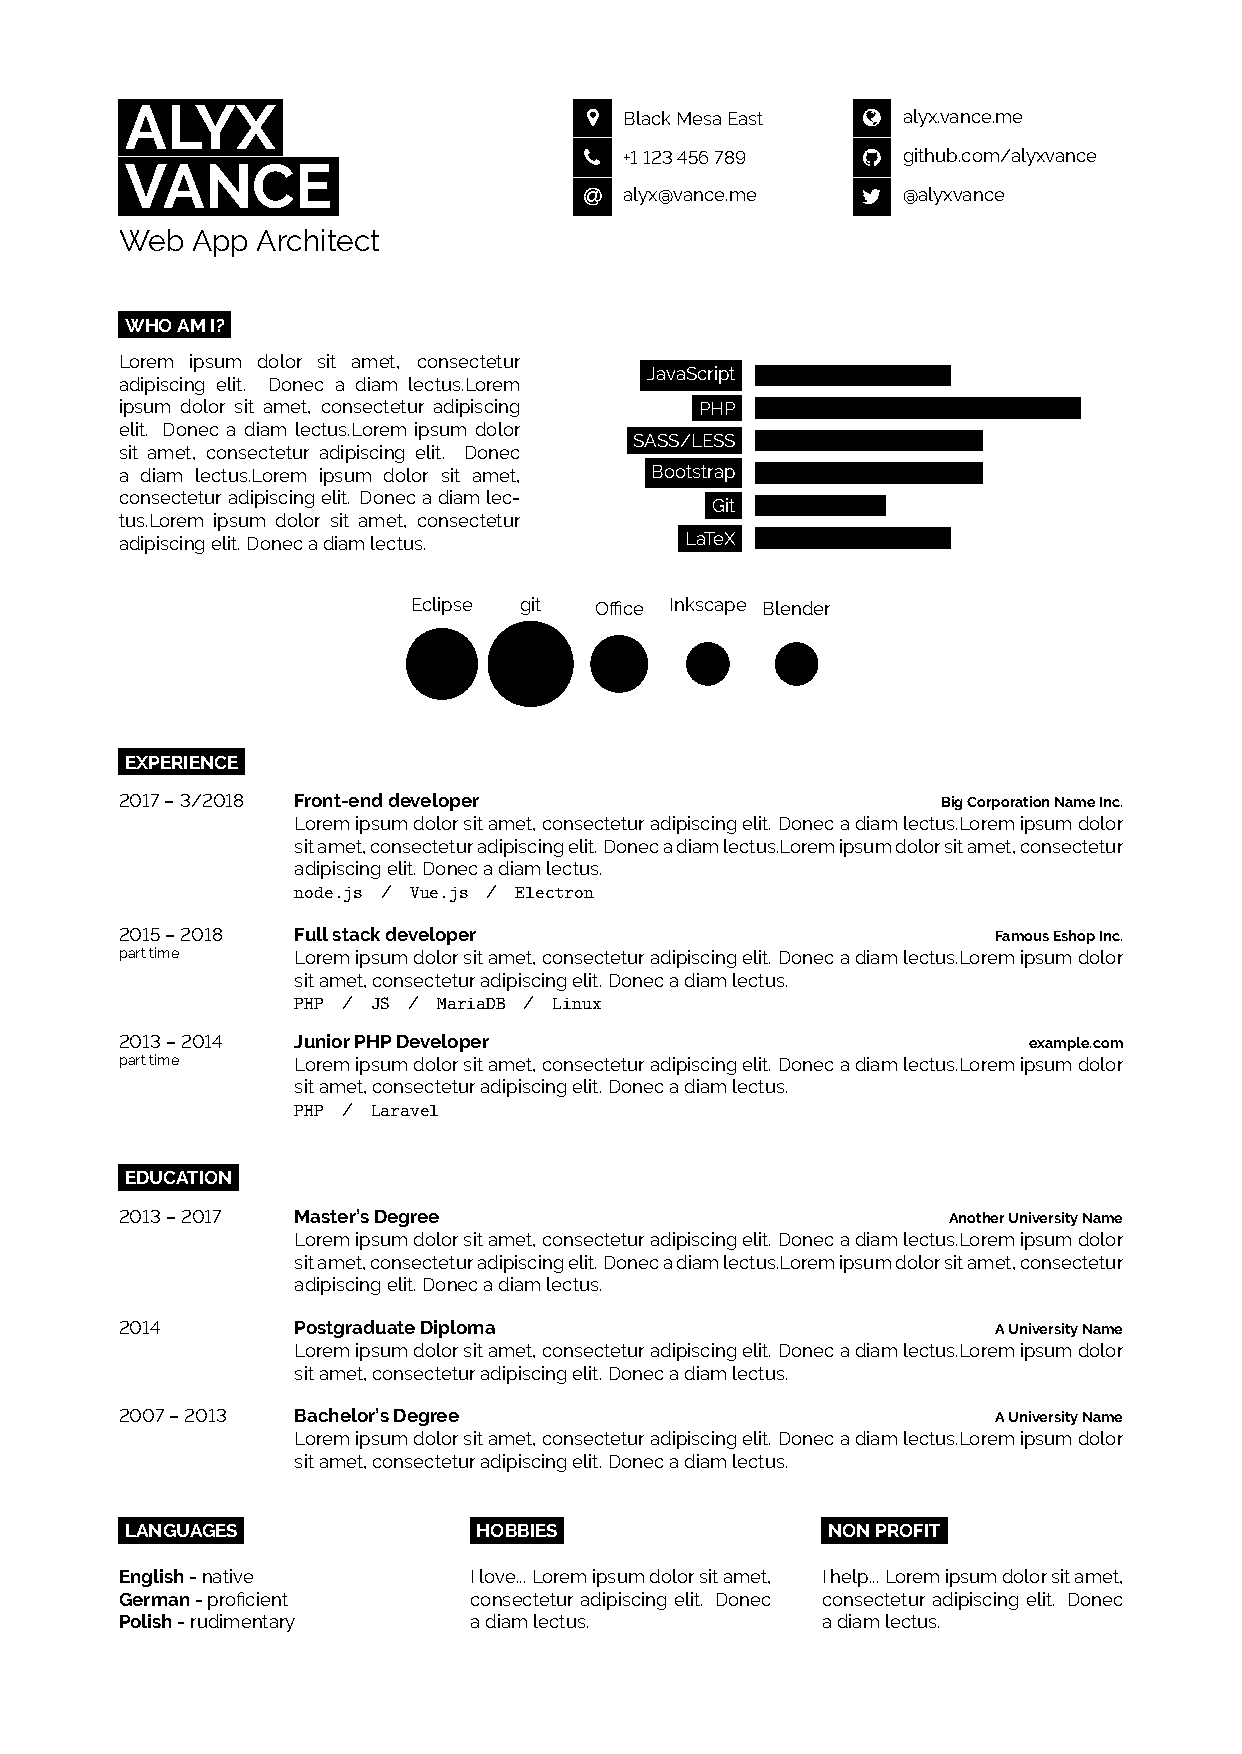
\includegraphics[width=0.8\textwidth]{../img/template_cv.pdf}}
          \caption{CV (\href{https://www.latextemplates.com/template/developer-cv}{source})}
        \end{figure}
    \column{.5\textwidth}
        \begin{figure}[h]
          \def\figurename{Exemple 2}
          \fbox{
\includegraphics[width=0.8\textwidth]{../img/template_master_thesis.pdf}}
          \caption{Mémoire (\href{https://www.overleaf.com/latex/templates/master-in-cybersecurity-be-thesis-template-ulb-unamur-ucl-he2b-slash-esi-helb-erm/ypmhcxmmtgkn}{source})}
        \end{figure}
  \end{columns}

  

\end{frame}
